\chapter{Konzept und Implementation}\label{ch:konzept}

Im Folgenden sollen die in \Cref{ch:grundlagen} beschriebenen Grundlagen und Entwurfsmuster genutzt werden und um anhand der in \Cref{ch:analyse} analysierten Komponenten ein Konzept sowie die dazugehörige Implementierung vorzustellen.

\section{Top-Level-Architektur}\label{sec:tla}

Um die in \Cref{sec:problem} aufgeführten strukturellen Problemen beheben zu können, wurde zu Beginn der Arbeit eine geeignete Ordner- und Applikationsstruktur festgelegt. Mit der Grundlage der erstellten Dialoglandkarte aus \Cref{sec:app-architecture-mindmap} und der Kenntnis der Datenbank-Framework aus \Cref{sec:couchbase-framework} konnte eine Top-Level-Architektur-Modell (TLA) erstellt werden. Dabei wurden die verschiedenen Aspekte der Anwendung weitestgehend unabhängige Komponenten unterteilt, die separat entwickelt werden können. Entsprechend dieser Unterteilung ließen sich die folgenden Komponenten ableiten, die anschließend in eigenen \texttt{Packages} implementiert wurden:

\begin{itemize}
    \item Im Root-Verzeichnis befinden sich Konfigurationsdateien des Build-Tools Gradle sowie Hilfsdateien, die nicht direkt zur Codebasis der App gehören. Außerdem befindet sich an dieser Stelle das Applikationsverzeichnis.
    \textbf{de.outputdd.android} beinhaltet in der obersten Applikationsebene globale Klassen, wie die \texttt{OutputApplication}, \texttt{MainActivity} und \texttt{GameService} Klasse. Diesen bilden die Basis der Applikation und stellen notwendige Funktionalität bereit, welche in allen Bereichen der App genutzt wird, wie unter anderem die Instanziierung der Repository-Objekte.
    \item \textbf{de.outputdd.android.common} stellt eine Reihe von Komponenten und Erweiterungen bereit, welche die bestehende Android-Bibliothek ergänzen, beispielsweise eine Ansammlung von \texttt{Extensions}\footnote{Extensions \url{https://kotlinlang.org/docs/extensions.html}} welche häufig wiederverwendet werden um die Lesbarkeit und Komplexität des Quellcodes zu verbessern.  
    \item \textbf{de.outputdd.android.game} umfasst die Funktionalitäten der Gamification. Dabei stehen generische Klassen für verschiedene Aufgaben-Typen des OUTPUT-Spiels bereit.
        \begin{itemize}
            \item \textbf{de.outputdd.android.game.observer} enthält alle für das Spiel eingesetzten Aufgaben, die eine Nutzer erfüllen kann. Diese werden von eigenständigen Klassen implementiert.
        \end{itemize} \newpage
    \item \textbf{de.outputdd.android.ui} ist die mächtigste Komponente, da sie die Fragmente aller Ansichten der App sowie die dafür notwendigen Views und Adapter kapselt. 
        \begin{itemize}
            \item \textbf{de.outputdd.android.ui.adapter} besteht aus generischen Klassen, welche in vielen Ansichten wiederverwendet werden um die \texttt{RecyclerView}\footnote{RecyclerView. \url{https://developer.android.com/guide/topics/ui/layout/recyclerview}}- sowie \texttt{Viewpager2}\footnote{Viewpager2. \url{https://developer.android.com/training/animation/screen-slide-2}}-Instanzen der App zu konfigurieren. Hinzu kommen eine Reihe von Binding-Adaptern\footnote{Binding-Adapter. \url{https://developer.android.com/topic/libraries/data-binding/binding-adapters}} die das Konzept von \texttt{Databinding} aus \Cref{subsec:databinding} um eigene Attribute erweitert.
            \item \textbf{de.outputdd.android.ui.dialog} umfasst die Dialog-Ansichten der App, welche als \texttt{BottomSheetDialogFragment}\footnote{BottomSheetDialogFragment. \newline \url{https://material.io/develop/android/components/bottom-sheet-dialog-fragment}} umgesetzt wurden.
            \item \textbf{de.outputdd.android.ui.feed} stellt alle Twitter-Funktionalitäten bereit, inklusive der Timeline-Ansicht und der Möglichkeit, neue Tweets zu erstellen.
            \item \textbf{de.outputdd.android.ui.game} beinhaltet alle Ansichten, die im Zusammenhang mit dem OUTOUT-Spiel stehen, darunter die Spieler-Registrierung, die Fortschrittsansicht und die Rangliste.
            \item \textbf{de.outputdd.android.ui.home} realisiert die Home-Ansicht der App, welche als Verknüpfung zwischen den verschiedenen Ansichten dient.
            \item \textbf{de.outputdd.android.ui.info} stellt die Ansichten der Info-View zur Verfügung, darunter die Lizenz-Ansicht, Danksagung aber auch die Informationen des Crowd-Monitorings und des Datenschutzes.
            \item \textbf{de.outputdd.android.ui.map} ist verantwortlich für die Kartenansicht der App, inklusive der Heatmap, Stände und Eroberungen.
            \item \textbf{de.outputdd.android.ui.program} beinhaltet den Veranstaltungsplan der Messe. Neben der Übersicht lassen die Beiträge auch nach Kategorie und Freitextsuche filtern. Eine Detailansicht gibt die vollständigen Informationen einer Veranstaltung wieder.
            \item \textbf{de.outputdd.android.ui.scan} realisiert die Ansicht des QR-Code-Scanners und der damit verbundenen Auswertung von gescannten Codes.
            \item \textbf{de.outputdd.android.ui.tutorial} stellt das App-Tutorial zur Verfügung, um dem Nutzer nach Installation der App in die verschiedenen Ansichten einzuführen.
            \item \textbf{de.outputdd.android.ui.widget} bietet eigene View-Klassen, die in den verschieden Layouts genutzt werden und die bestehenden View-Klassen der Android Bibliothek um weitere Funktionen ergänzen.
        \end{itemize}
\end{itemize}

\newpage

\section{Programmier-Richtlinien}\label{sec:guidelines}

Um das Projekt bestmöglich auf die Weiterentwicklung vorzubereiten wurden eine Reihe von Vorkehrungen getroffen. 
\newline Da die Android-App potenziell von mehreren Nutzern auf den verschiedenen Betriebssystemen entwickelt werden kann, wurde eine entsprechende Konfigurationsdatei ergänzt, welche dafür sorgt, dass die Quellcode-Dateien über konsistente Zeilenenden verfügen. Anhand einer \texttt{.gitattributes}-Datei im Root-Verzeichnis des Repository werden Dateien beim \enquote{Checkout} von Git automatisch konvertiert. Dadurch können fehlerhafte Änderungs-Anzeigen vermieden und zugleich eine potenzielle Fehlerquelle ausgeschlossen werden.\newline Um jede Datei mit einem deskriptiven Kommentar auszustatten, wurde sich im Projektteam für die Einführung eines Copyright-Hinweis entschieden. Um Diskrepanzen zwischen dem Dateinamen und dem Hinweis zu verhindern, wurde im Rahmen des Projektes ein Copyright-Template erstellt, um anschließend im Projekt eingebunden und auf alle Dateien angewendet werden zu können. Wie in \Cref{fig:copyright} dargestellt, enthält das Copyright-Template zusätzlich zu Hinweisen und Links über die Herkunft des Quellcodes auch einen Link zu den Richtlinien der Weiterentwicklung. Das Template ist dabei bewusst so ausgelegt, dass sich mehrere Autoren inklusive ihrer Kontaktinformationen eintragen können. Letzteres ist wichtig, da sich im Projektteam noch nicht auf eine Lizenzierung der Apps unter Open-Source-Lizenzen festgelegt wurde und daher der Quellcode unter das Kopierrecht des Autors fallen. Wenn eine Weiterverwendung des Codes über den ursprünglich dafür bestimmten Rahmen stattfindet, so können die Autoren hierüber kontaktiert werden.

\begin{figure}[H]
    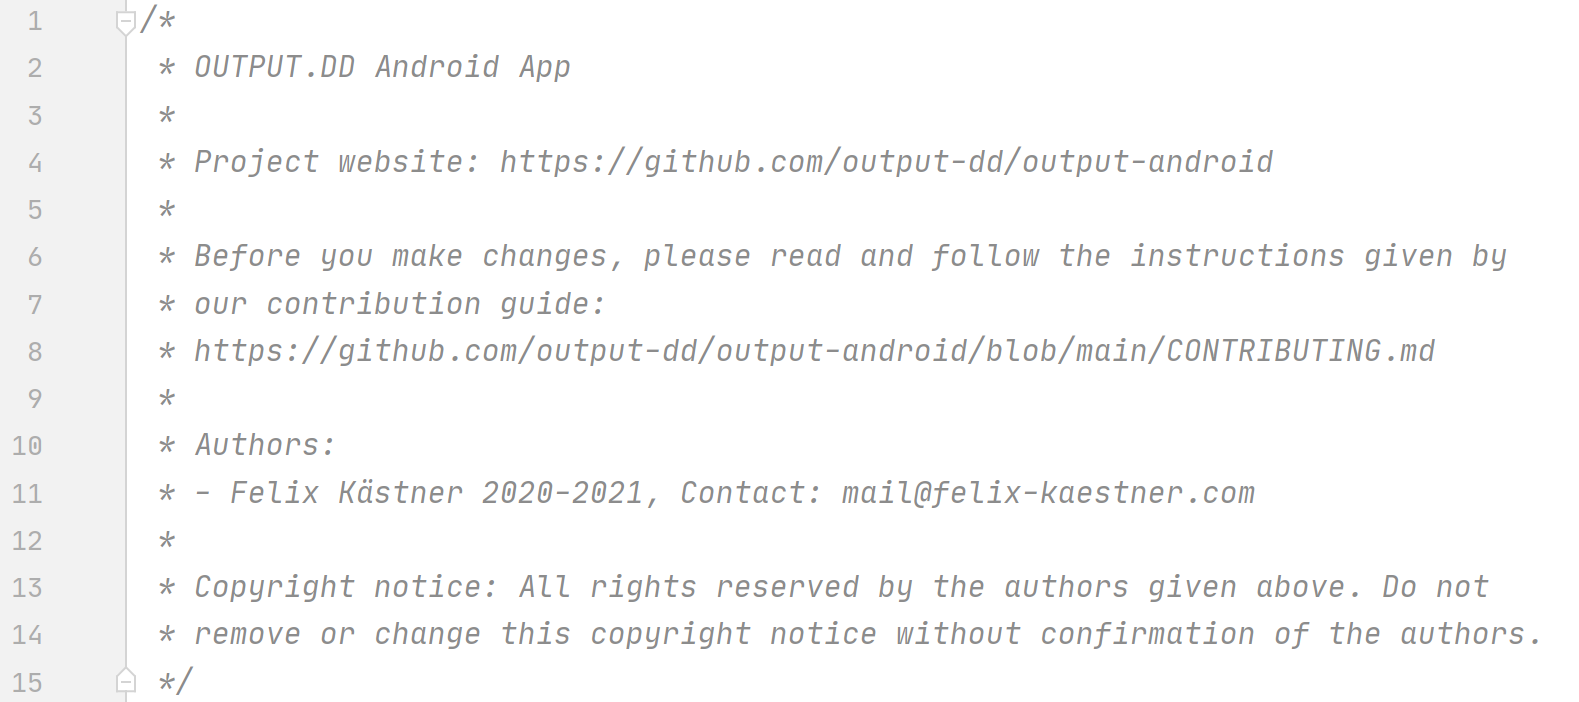
\includegraphics[width=1\linewidth]{41-copyright.png}
    \caption{Das Copyright-Template des Quellcodes.}\label{fig:copyright}
\end{figure}

Um die Probleme der Codequalität der vorhergehenden App zu vermeiden, wird das in Android-Studio integrierte Analyse und Formatierungs-Werkzeug genutzt, um die Codequalität aufrechtzuerhalten. Diese wird bei jedem Commit geprüft und dem Entwickler als Warnung anzeigt. Zukünftige Entwickler sind dazu angehalten diese Meldungen nicht zu ignorieren, sondern ihnen stattdessen Aufmerksamkeit zu schenken und entsprechende Verbesserungen durchzuführen. Durch das Interaktions-Menü welches in Android Studio integriert ist, wird es dem Entwickler erleichtert, auf Feedback einzugehen und Anpassungen schnell und unkompliziert durchzuführen.

\newpage

\section{Umsetzung der Ansichten}\label{sec:view-implementation}

Mit der vorliegenden Konzeption zur Unterteilung der Komponenten und den etablierten Richtlinien begann die Umsetzung der Ansichten. Die Implementation der Ansichten fand dabei zunächst unabhängig vom Datenbank-Backend statt. Stattdessen wurden Beispieldaten verwendet, um die Views zu generieren. Gleichzeitig wurde allerdings bereits großer Wert auf die Strukturierung der ViewModels gelegt, um im späteren Verlauf die Beispieldaten auf einfache Weise durch das Datenbank-Backend ergänzen zu können. Dadurch ergaben sich einige Vorteile im Entwicklungsprozess, da die Ansichten in einem schnelleren Entwicklungszyklus erstellt werden konnten und die notwendige Separation leichter umsetzbar war. Im Folgenden konnte bereits nach wenigen Wochen die Benutzeroberfläche zwischen der iOS und Android App abgeglichen werden.

\subsection{Erstellung von Fragments}\label{subsec:fragments}

Um die in \Cref{subsec:viewbinding} und \Cref{subsec:databinding} vorgestellten Konzepte von Viewbinding und Databinding zu Nutzen, empfiehlt die offizielle Dokumentation\footnote{Viewbinding in Fragments. \url{https://developer.android.com/topic/libraries/view-binding\#fragments}} die Nutzung von \texttt{Backing Properties}\footnote{Backing Properties. \url{https://kotlinlang.org/docs/reference/properties.html\#backing-properties}} in Kotlin. Dabei entsteht inhärent eine gewisse Verbosität. Damit diese Umstände vermieden werden konnte, wurde eine entsprechende Lösung anhand der Klasse \texttt{AutoClearedValue} eingeführt. Diese Klasse beobachtet den Lebenszyklus des Fragments und invalidiert Zugriffe, sobald sich das Fragment im \texttt{onDestroy}-Status befindet. Mittels einer \texttt{Extension}\footnote{Extension. \url{https://kotlinlang.org/docs/extensions.html}} konnte die Verwendung der Klasse über \texttt{Delegated Properties}\footnote{Delegated Properties. \url{https://kotlinlang.org/docs/reference/delegated-properties.html}} bereitgestellt werden. Anhand des in \Cref{subsec:delegation} beschrieben Pattern von Delegation kann die entsprechende Variable in die Nutzung innerhalb der Fragment-Klasse eingebunden werden. Da es sich im Allgemeinen empfiehlt während der \texttt{onCreateView} eines Fragments nur äußerst sparsame Operationen vorzunehmen und stattdessen komplexe Anwendungslogik in die \texttt{onViewCreated} auszulagern, wird die entsprechende Layout-Datei dem Konstruktur der Klasse \texttt{Fragment} übergeben und die Viewbinding-Instanz in der \texttt{onViewCreated}-Methode gebunden. Daraus ergibt sich folgender Aufbau der Ansichten:

\begin{figure}[H]
    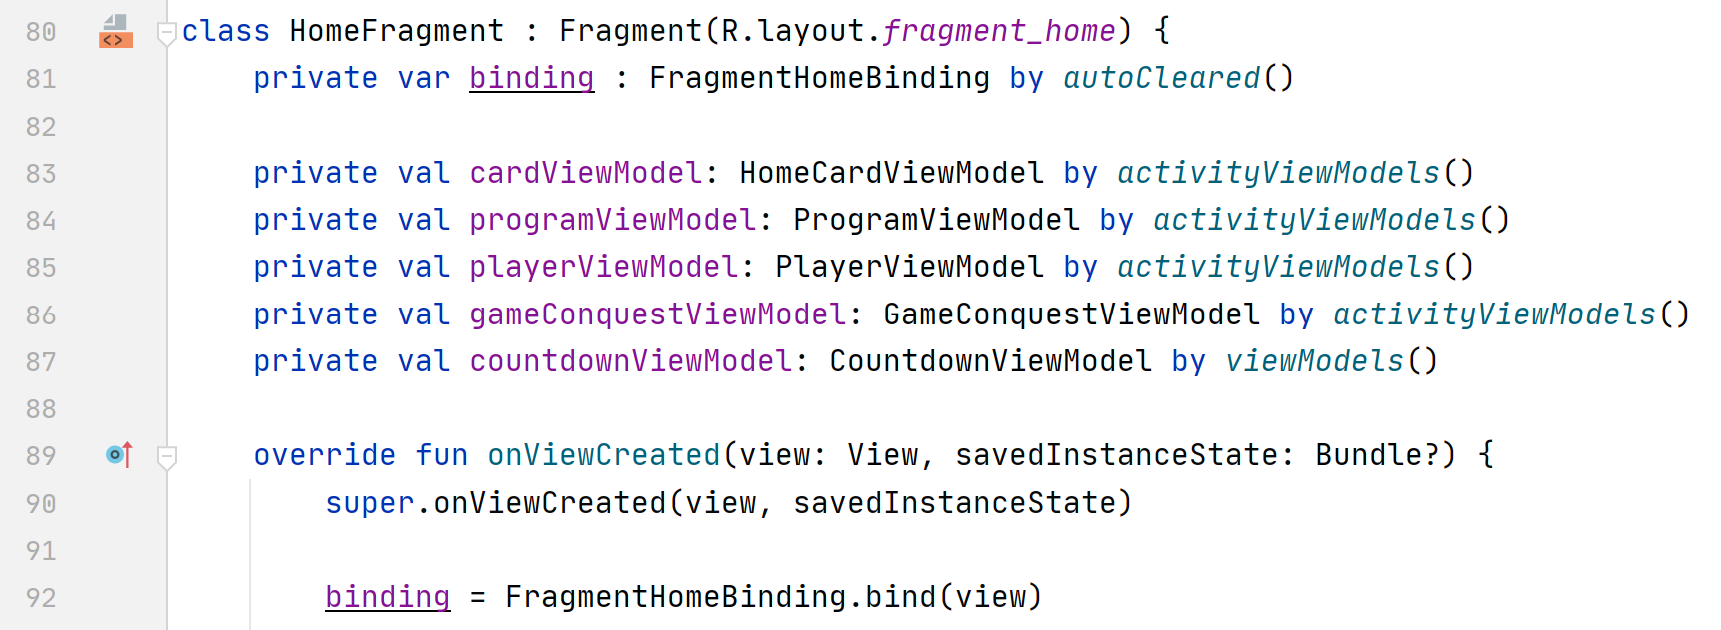
\includegraphics[width=1\linewidth]{42-fragment.png}
    \caption{Ausschnitt des Quellcodes des Home-Fragments.}\label{fig:fragment}
\end{figure}

\newpage

In \Cref{fig:fragment} zu sehen ist ein Ausschnitt des Quellcodes der Home-Ansicht. Dabei zu sehen ist die Nutzung des in \Cref{subsec:delegation} vorgestellten Prinzips von Delegation zur Bereitstellung der Klassen-Variablen. Neben der Verwendung der Methode \texttt{autoCleared()} zur Erstellung einer Instanz der Klasse \texttt{AutoClearedValue} wie oben beschrieben, ist auch die Delegation zur Erstellung von ViewModel-Instanzen zu sehen. Dies geschieht mittels der Methoden \texttt{viewModels()} und \texttt{activityViewModels()} die als Teil von Android KTX\footnote{Android KTX \url{https://developer.android.com/kotlin/ktx}} zur Verfügung stehen.

\subsection{Verwendung von Viewmodels}\label{subsec:viewmodel-implementation}

Für die Bereitstellung von Daten mittels des entwickelten Datenbank-Frameworks wurde auf \texttt{Kotlin Coroutines}\footnote{Coroutines. \url{https://kotlinlang.org/docs/coroutines-overview.html}} zurückgegriffen. Couchbase bietet die Möglichkeit zur Erstellung sogenannter \texttt{Live Query}\footnote{Live Query. \newline \url{https://docs.couchbase.com/couchbase-lite/current/android/learn/java-android-query-live.html}}-Objekte. Dabei wird ein \texttt{Listener} auf einer beliebigen Datenbankabfrage abgewendet. Sobald sich im Folgenden das Resultat der Datenbankabfrage ändert, wird ein entsprechender \texttt{Callback} ausgeführt. Diese Funktionalität wurde seitens des Datenbank-Frameworks gekapselt und im Allgemeinen unter den \texttt{addOnChangeListener}-Funktionen der Repository-Klasse zur Verfügung gestellt. Des Weiteren lässt sich diese Callback-basierte Asynchronität in einen asynchronen Datenfluss umwandeln. Kotlin führt dazu im Rahmen von \texttt{Coroutines} eine Datenstruktur für die Verwendung von asynchronen Datenfüssen namens \texttt{Flow}\footnote{Asynchronous Flow. \url{https://kotlinlang.org/docs/flow.html}} ein. Das Prinzip eines solchen Datenflusses ist äquivalent zu bekannten Lösungen wie \texttt{RxJava}\footnote{RxJava \url{https://github.com/ReactiveX/RxJava}}. Damit bietet \texttt{Flow} die Grundlage für asynchrone und Event-basierte Programmierung in Kotlin. Ein großer Vorteil von \texttt{Flow} ist das die Verarbeitung von Elementen ausgesetzt werden kann und in diesem Zustand den Main-Thread der Applikation, welcher für die UI zuständig ist, nicht blockiert. Ein weiterer Vorteil von \texttt{Flow} ist, dass diese sogenannte \enquote{cold streams} repräsentieren. Dabei werden Elemente erst transferiert, sobald ein entsprechender Empfänger vorhanden ist und diese verarbeitet. Im Falle der Android-App bedeutet dieser Sachverhalt, das Objekte erste bei entsprechender Ansicht in App von der Datenbank geladen werden. Die Verarbeitung der Elemente eines \texttt{Flow} geschieht wie auch die Ausführung einer \texttt{Coroutine} in einem entsprechenden Kontext. Dieser Kontext ist verantwortlich für die Koordination der Ausführung. Für den \texttt{CoroutineContext} stehen in der Android-Platform potenziell mehrere Optionen zur Verfügung, die für unterschiedliche Anwendungsszenarien geeignet sind. 

\begin{itemize}
    \item \textbf{Dispatchers.Default} bildet den Standardwert, welcher automatisch genutzt wird, sollte kein anderer \texttt{CoroutineContext} explizit angegeben werden. Dieser Kontext sollte nur zu Testzwecken genutzt werden und die explizite Zuweisung eines Kontext bevorzugt werden.
    \item \textbf{Dispatchers.Main} führt \texttt{Coroutines} auf dem Main-Thread der Applikation aus, der für die UI zuständig ist. In diesem Fall handelt es sich hierbei um einen einzelnen Thread, der die Aufgaben sequentiell bearbeitet. Für Android sollte stattdessen die Benutzung von \texttt{Dispatchers.Main.immediate} bevorzugt werden.
    \item \textbf{Dispatchers.Main.immediate} ist eine Erweiterung des \texttt{Dispatchers.Main} der lediglich auf der JVM und Android nutzbar ist. Dabei werden Aufgaben unverzüglich ausgeführt. Dieser Kontext sollte daher für Operationen genutzt werden, die im direkten Zusammenhang mit der UI stehen, wie beispielsweise die Durchführung eines HTTP-Request zur Registrierung des Spielers. \newpage
    \item \textbf{Dispatchers.Unconfined} gibt keine Aussage über die Ausführung. Stattdessen wird der aktuelle Thread für die Ausführung genutzt ohne jegliche Richtlinien zu setzen. Dieser unspezifische Kontext sollte ebenso vermieden werden.
    \item \textbf{Dispatchers.IO} führt Aufgaben auf einem Hintergrund-Prozess aus. Das kann Vorteilhaft sein um blockierende Aufrufe wie das Lesen von Dateien oder den Zugriff auf die Datenbank durchzuführen. Der Kontext verwendet dazu einen geteilten \enquote{Pool} von Threads die für die Ausführung herangezogen werden. Weitere Threads können bei Bedarf erstellt und nach Verwendung zerstört werden. 
\end{itemize}

Entsprechend ergibt sich für die Verwendung von \texttt{Coroutines} in ViewModels die Nutzung von \textbf{Dispatchers.Main.immediate} für die Deklaration von Methoden, welche direkt von der View aufgerufen werden sollen sowie \textbf{Dispatchers.IO} für Generierung eines \texttt{Flow}, welcher eine konstante Aktualisierung von Elemente (wie den Events der Programm-Ansicht) im Hintergrund ausführen soll. \newline Um die Elemente eines solchen Datenstroms anschließend nutzen zu können, werden diese in ein \texttt{LiveData}\footnote{LiveData. \url{https://developer.android.com/topic/libraries/architecture/livedata}}-Objekt konvertiert. \Cref{fig:viewmodel} zeigt die daraus resultierende Definition eines ViewModels in der App.

\begin{figure}[H]
    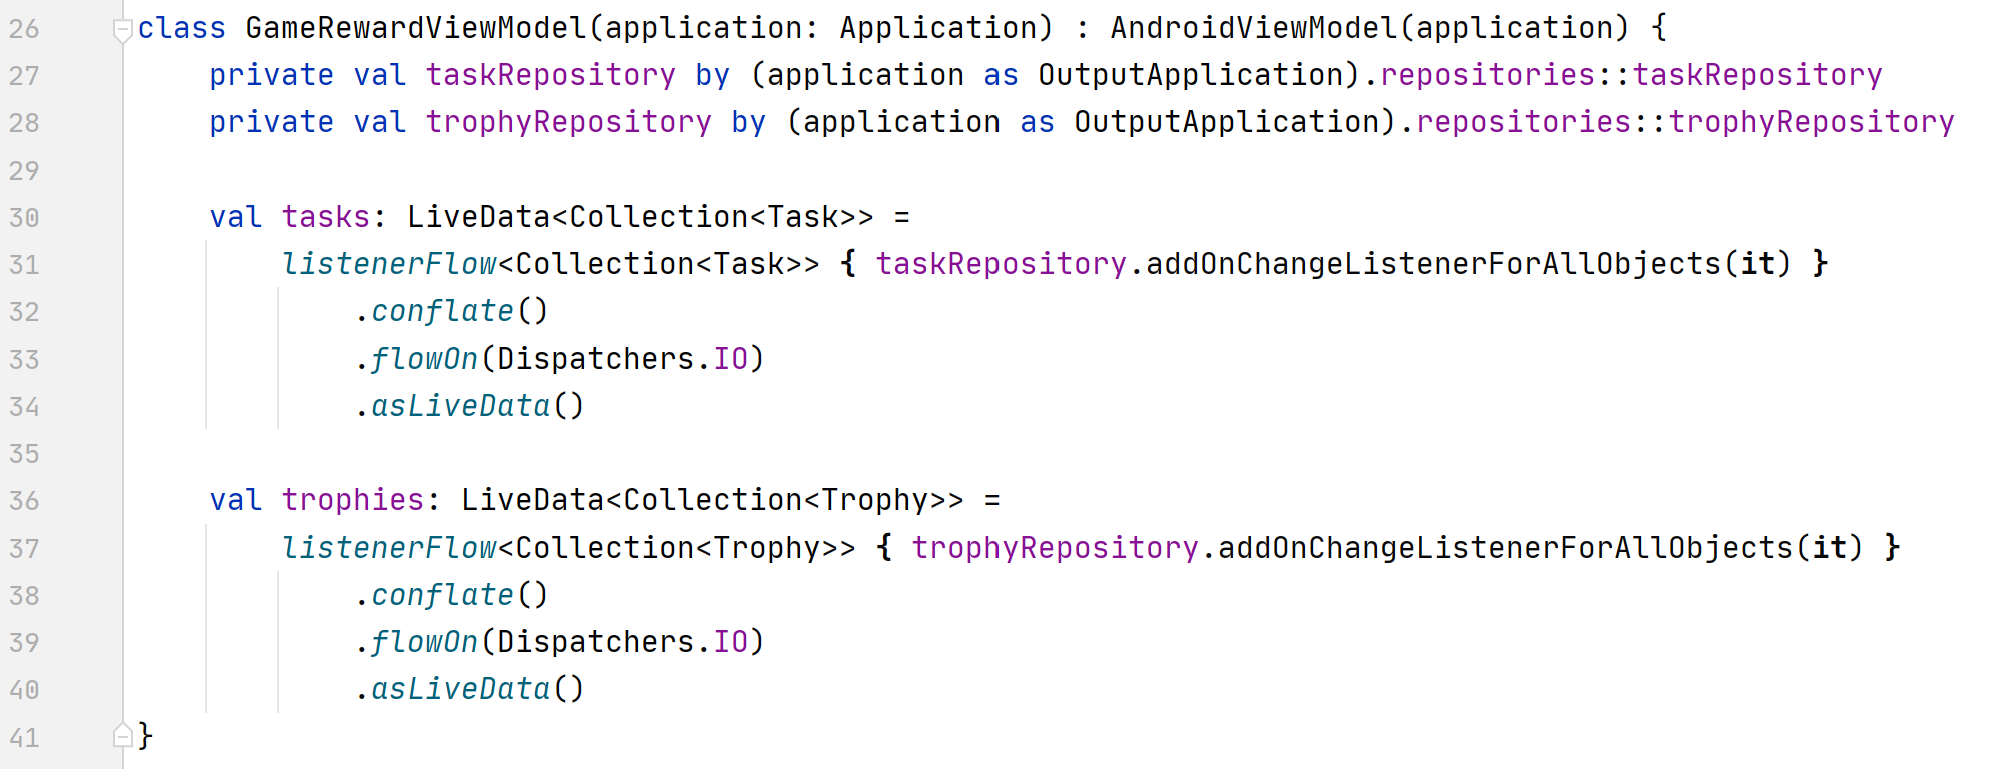
\includegraphics[width=1\linewidth]{43-viewmodel.png}
    \caption{Erstellung von ViewModels.}\label{fig:viewmodel}
\end{figure}

Die \texttt{LiveData}-Objekte können im folgenden genutzt werden, um die Ansichten zu erstellen. Dabei werden die Objekte nach dem in \Cref{sub:observer} beschriebenen Observer-Entwurfsmuster überwacht. Sobald sich im Folgenden die Daten dieser Objekte ändert, wird eine Aktualisierung der Ansicht durchgeführt. Dies geschieht im Falle der Verwendung von \hyperref[subsec:databinding]{Databinding} automatisch wie in \Cref{fig:fragment-viewmodel} anhand des \texttt{PlayerViewModel} zu sehen, welches automatisch die Spielansicht aktualisiert oder im Falle einer Listenansicht durch die Weitergabe der Objekte durch das Fragment, wie in \Cref{fig:fragment-viewmodel} anhand des \texttt{GameRewardViewModel} zu sehen. Bei letzterem geschieht die Generierung der Darstellung einzelner Elemente wie in \Cref{fig:databinding} und \Cref{lst:databinding} zu sehen.

\begin{figure}[H]
    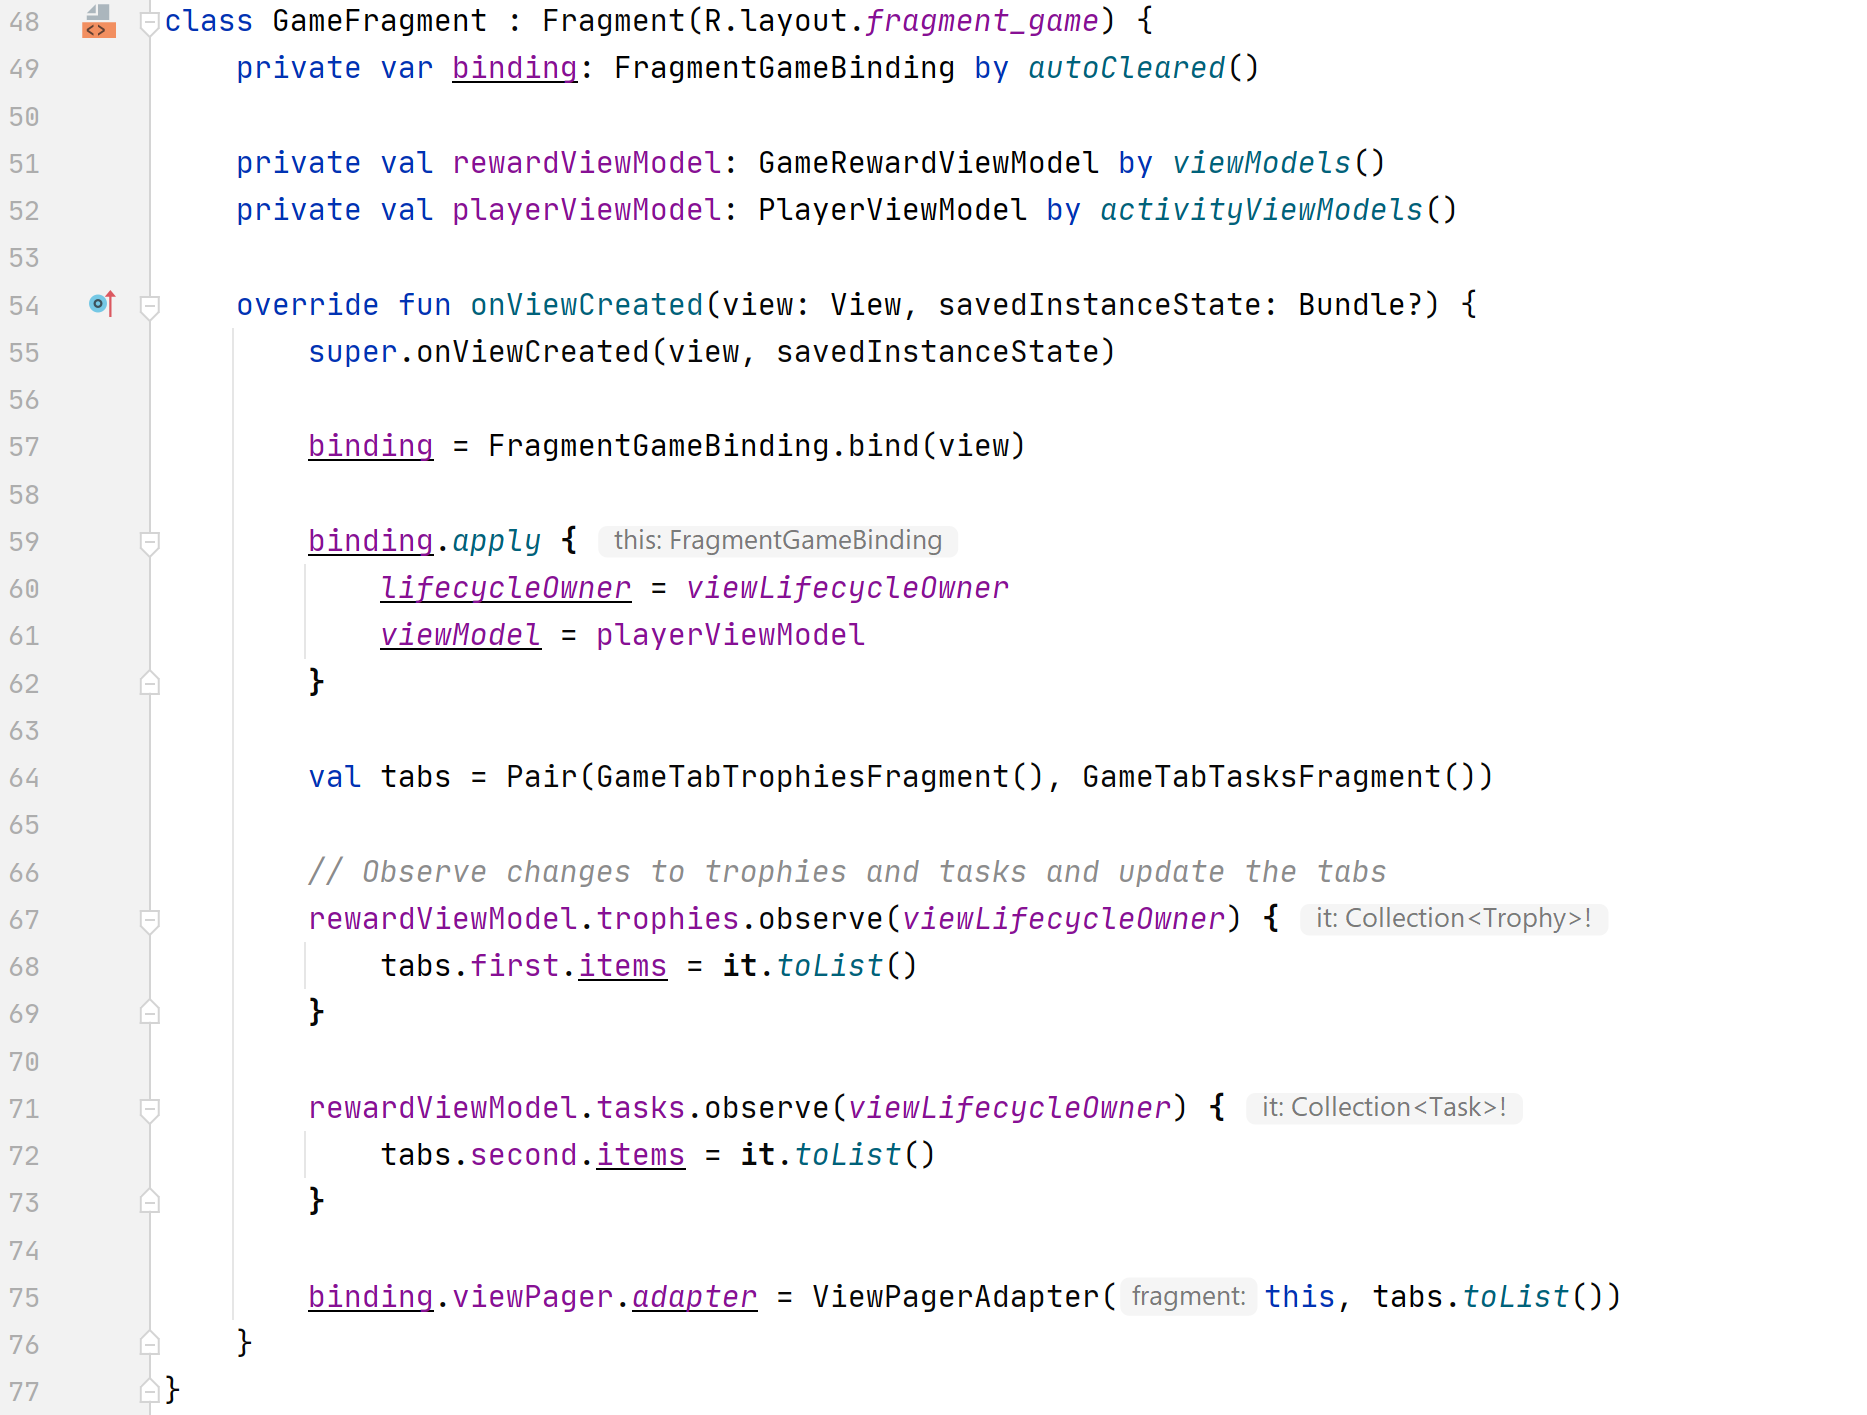
\includegraphics[width=1\linewidth]{44-fragment-viewmodel.png}
    \caption{Nutzung von ViewModels.}\label{fig:fragment-viewmodel}
\end{figure}

\subsection{Definition der Ansichten}\label{subsection:views}

Mittels der in \Cref{subsec:fragments} und \Cref{subsec:viewmodel-implementation} vorgestellten Konzepte und Implementierungen konnten die Ansichten der App definiert werden. \Cref{fig:screens} zeigt die 5 Hauptansichten der App. Weitere Ansichten wurden entsprechend der Dialoglandkarte aus \Cref{sec:app-architecture-mindmap} umgesetzt. Der Aufbau der Ansicht orientiert sich an der Implementation der vorangegangenen Jahre. Allerdings wurde im Rahmen der Neuimplementation auch eine Modernisierung der Benutzeroberfläche durchgeführt. Darunter ergeben sich auch neue Funktionen wie ein dunkles Design, welches automatisch durch die Systemeinstellung des Nutzers aktiviert wird und bei Dunkelheit die Augen vor zu viel Helligkeit schützt. Außerdem wurde eine Reihe von Animationen eingeführt, welche die Nutzererfahrung steigern und die Nutzerinteraktion unterstützen. Im Sinne der Grundprinzipien des Usability Engineerings wurde ebenso auf die Platzierung von Interaktionselementen in der unteren Hälfte des Bildschirms geachtet, um für den Nutzer leichter erreichbar zu sein. Für eine konsistente Nutzererfahrung sorgt auch die Modularisierung von UI-Komponenten, welche für mehrere Ansichten in der App wiederverwendet wurden. Zur Bereitstellung eines Themes wurde auf ein Theme der \texttt{Material Design}\footnote{Material Design. \url{https://material.io/resources/build-a-material-theme}} Bibliothek als Grundlage zurückgegriffen, um dem Nutzer eine plattformspezifische Erfahrung zu bieten. Gleichzeitig wurde bei der Auswahl der Formen, Farben und Fonts auf die Vorgaben aus der OUTPUD.DD Corporate Identity geachtet. Neben der Neuimplementation des gesamten UI, inklusive komplexerer Ansichten wie die \enquote{Reward-Ansicht} mit einer Konfetti-Animation, wurde in der Kartenansicht \texttt{Google Maps} durch \texttt{Mapbox}\footnote{Mapbox. \url{https://www.mapbox.com/}} ersetzt, da das Mapbox-Framework durch seine Nutzerfreundlichkeit und einfachen Handhabung im Projektteam befürwortet wurde. Auch die Twitter-Ansicht wurde erneuert. Statt der Verwendung des mittlerweile eingestellten Twitter-Frameworks wurde eine rein auf HTML basierende Lösung entwickelt. Dabei wird ein HTML-Template in einer \texttt{Webview}\footnote{Webview. \url{https://developer.android.com/reference/android/webkit/WebView}} dargestellt. Durch diese Implementierung wird kein API-Schlüssel benötigt und konnte zugleich eine zukunftssichere Lösung geschaffen werden.

\begin{figure}[H]
    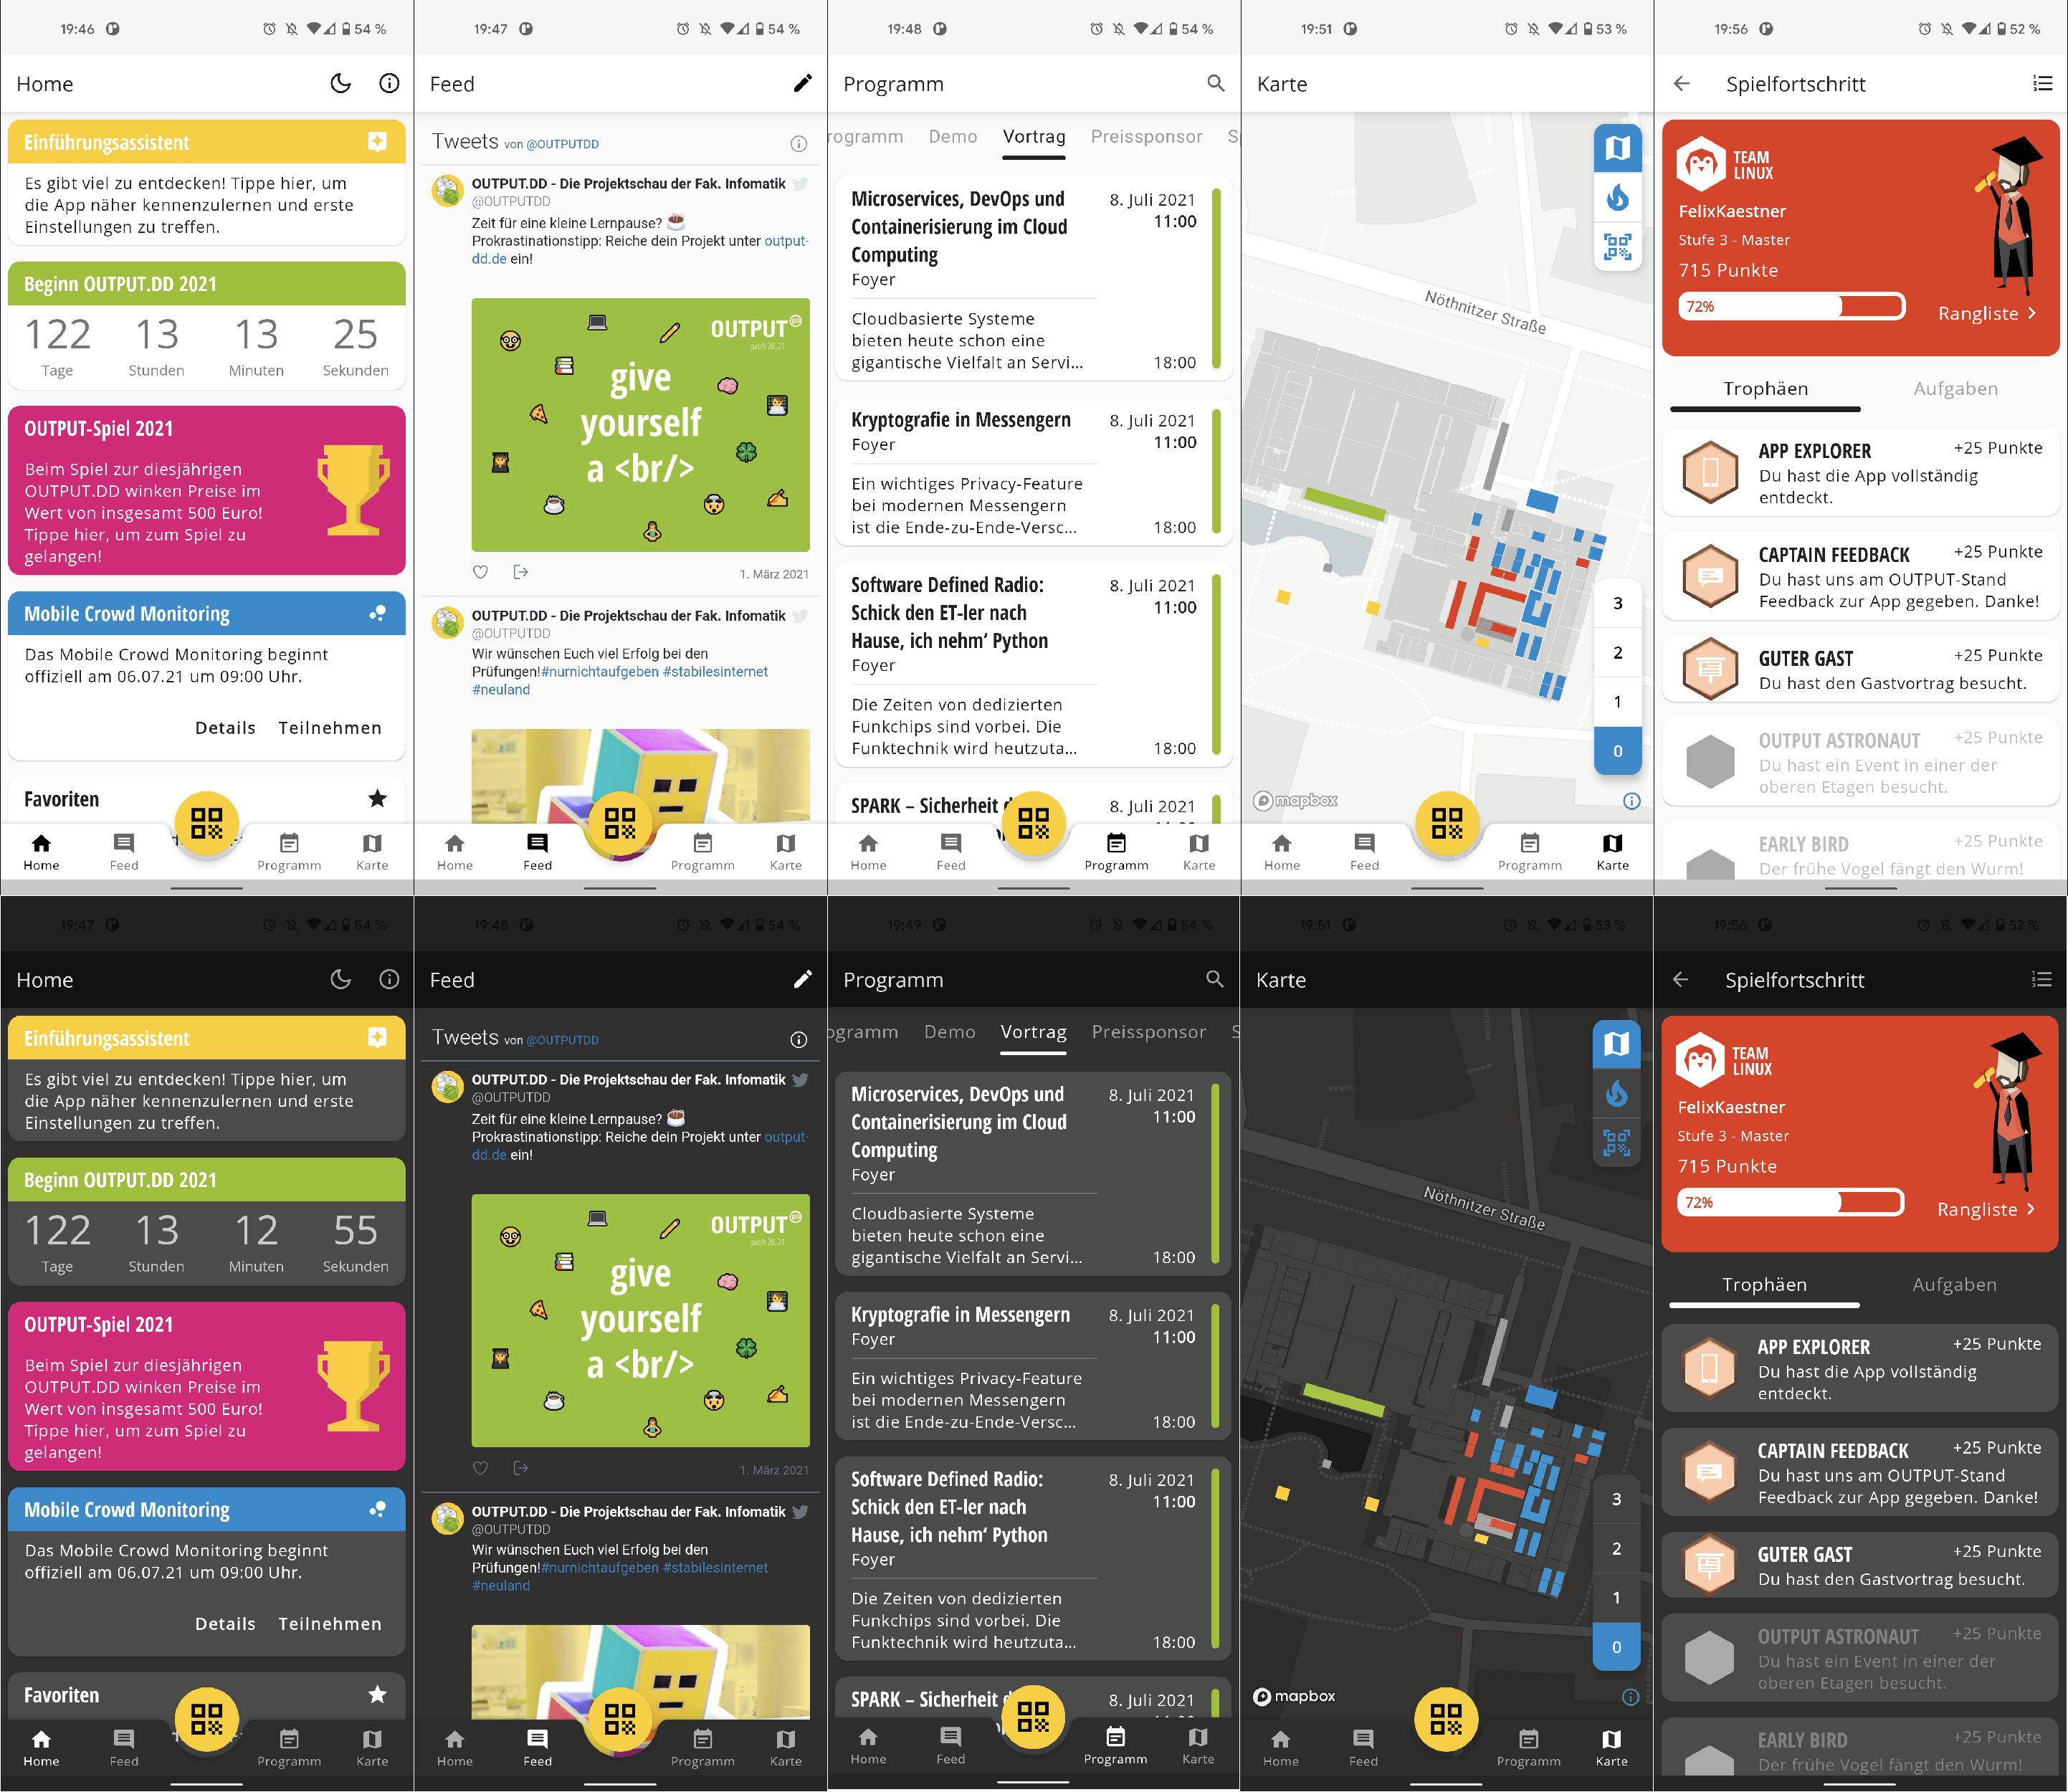
\includegraphics[width=1\linewidth]{45-screens.pdf}
    \caption{Die 5 Hauptansichten der App.}\label{fig:screens}
\end{figure}

\newpage

\section{Anbindung der Gamification}

Ein zentraler Bestandteil der App ist das darin enthaltene Spiel. Nutzer können sich einen Spieler mit einem eigenen Charakter erstellen und gegen andere Spieler antreten. Neben einer Reihe von Aufgaben innerhalb der App können QR-Codes gescannt werden um Errungenschaften freizuschalten. Grundsätzlich wird dabei zwischen Aufgaben und Trophäen unterschieden. Während Aufgaben zum Teil wiederholt abgeschlossen werden können, ist es nur einmalig möglich eine Trophäe zu erhalten. Für jede Errungenschaft bekommt der Spieler \texttt{xp}, welche seinen Charakter auf eine neue Stufe aufsteigen lassen und der Avatar des Spielers verändert wird. Gleichzeitig erhält der Spieler aber auch Punkte, anhand welcher der Spieler auf der Rangliste eingeordnet wird und sich mit anderen Spielern vergleichen kann. Im Allgemeinen dient die Einbringung von Gamification zur Steigerung der Interaktion eines Messebesuchers. Zur Implementation der Gamification innerhalb der App wurden die bestehenden Aufgaben und Trophäen analysiert und anschließend ein Konzept erstellt, um diese umzusetzen. Aus diesem Grund wurde eine Übersicht erstellt, welche die entsprechenden Kriterien beinhaltet, die ein Nutzer erfüllen muss, um die jeweilige Errungenschaft zu erhalten. Anhand unserer Analyse konnten zwei Kategorien ermittelt werden.

\begin{itemize}
    \item \textbf{Datenbasierte} Errungenschaften werden durch die Erstellung von bestimmten Objekten in der Datenbank erreicht. Beispiele hierfür sind das Speichern eines gescannten QR-Codes oder die Registrierung eines neuen Spielers.
    \item \textbf{Interaktionsbasierte} Errungenschaften werden durch die Interaktion mit bestimmten Elementen der App erreicht, welche keine direkte Änderung von Daten innerhalb der Datenbank bewirken. Beispiele hierfür sind das Aufrufen von einzelnen Ansichten oder die Änderung des Modus der Kartenansicht.
\end{itemize}

Die Freischaltung von Errungenschaften kann hierbei als Observation von Nutzeraktionen gesehen werden, welche gemäß dem in \Cref{sub:observer} beschrieben Entwurfsmuster durchgeführt und im Hintergrund ausgeführt wird. Somit arbeiten die observierenden Komponenten selbstständig und entscheiden bei Benachrichtigung durch ein Ereignis, ob die entsprechende Errungenschaft freigeschaltet werden soll. Durch dieses Paradigma konnte die Gamification sehr gut von der restlichen Anwendungslogik der App separiert werden. 

\subsection{Implementation von datenbasierten Errungenschaften}\label{subsection:gamification-repository-listener}

Da die Freischaltung von datenbasierte Errungenschaften direkt von der Änderung bestimmter Datenmodelle innerhalb der Datenbank abhängt, wurde äquivalent zur Umsetzung der Viewmodels aus \Cref{subsec:viewmodel-implementation} auf die Verwendung von \texttt{Flow} zurückgegriffen. Dabei werden entsprechende Datenbank-Listener für die jeweiligen Datenmodelle genutzt, welche anschließend in einen asynchronen Datenstrom transformiert werden. Ein solcher \texttt{Flow} kann im Folgenden genutzt werden, um bei jedem eintreffenden Objekte zu prüfen, ob die Errungenschaft freigeschaltet werden soll. Der vollständige Algorithmus für den Lebenszyklus eines Observer ist in \Cref{fig:repository-listener} abgebildet, wobei die Nutzung eines asynchronen Datenstrom in Blau und die Freischaltung der Errungenschaft in Grün markiert ist.  

\begin{figure}[H]
    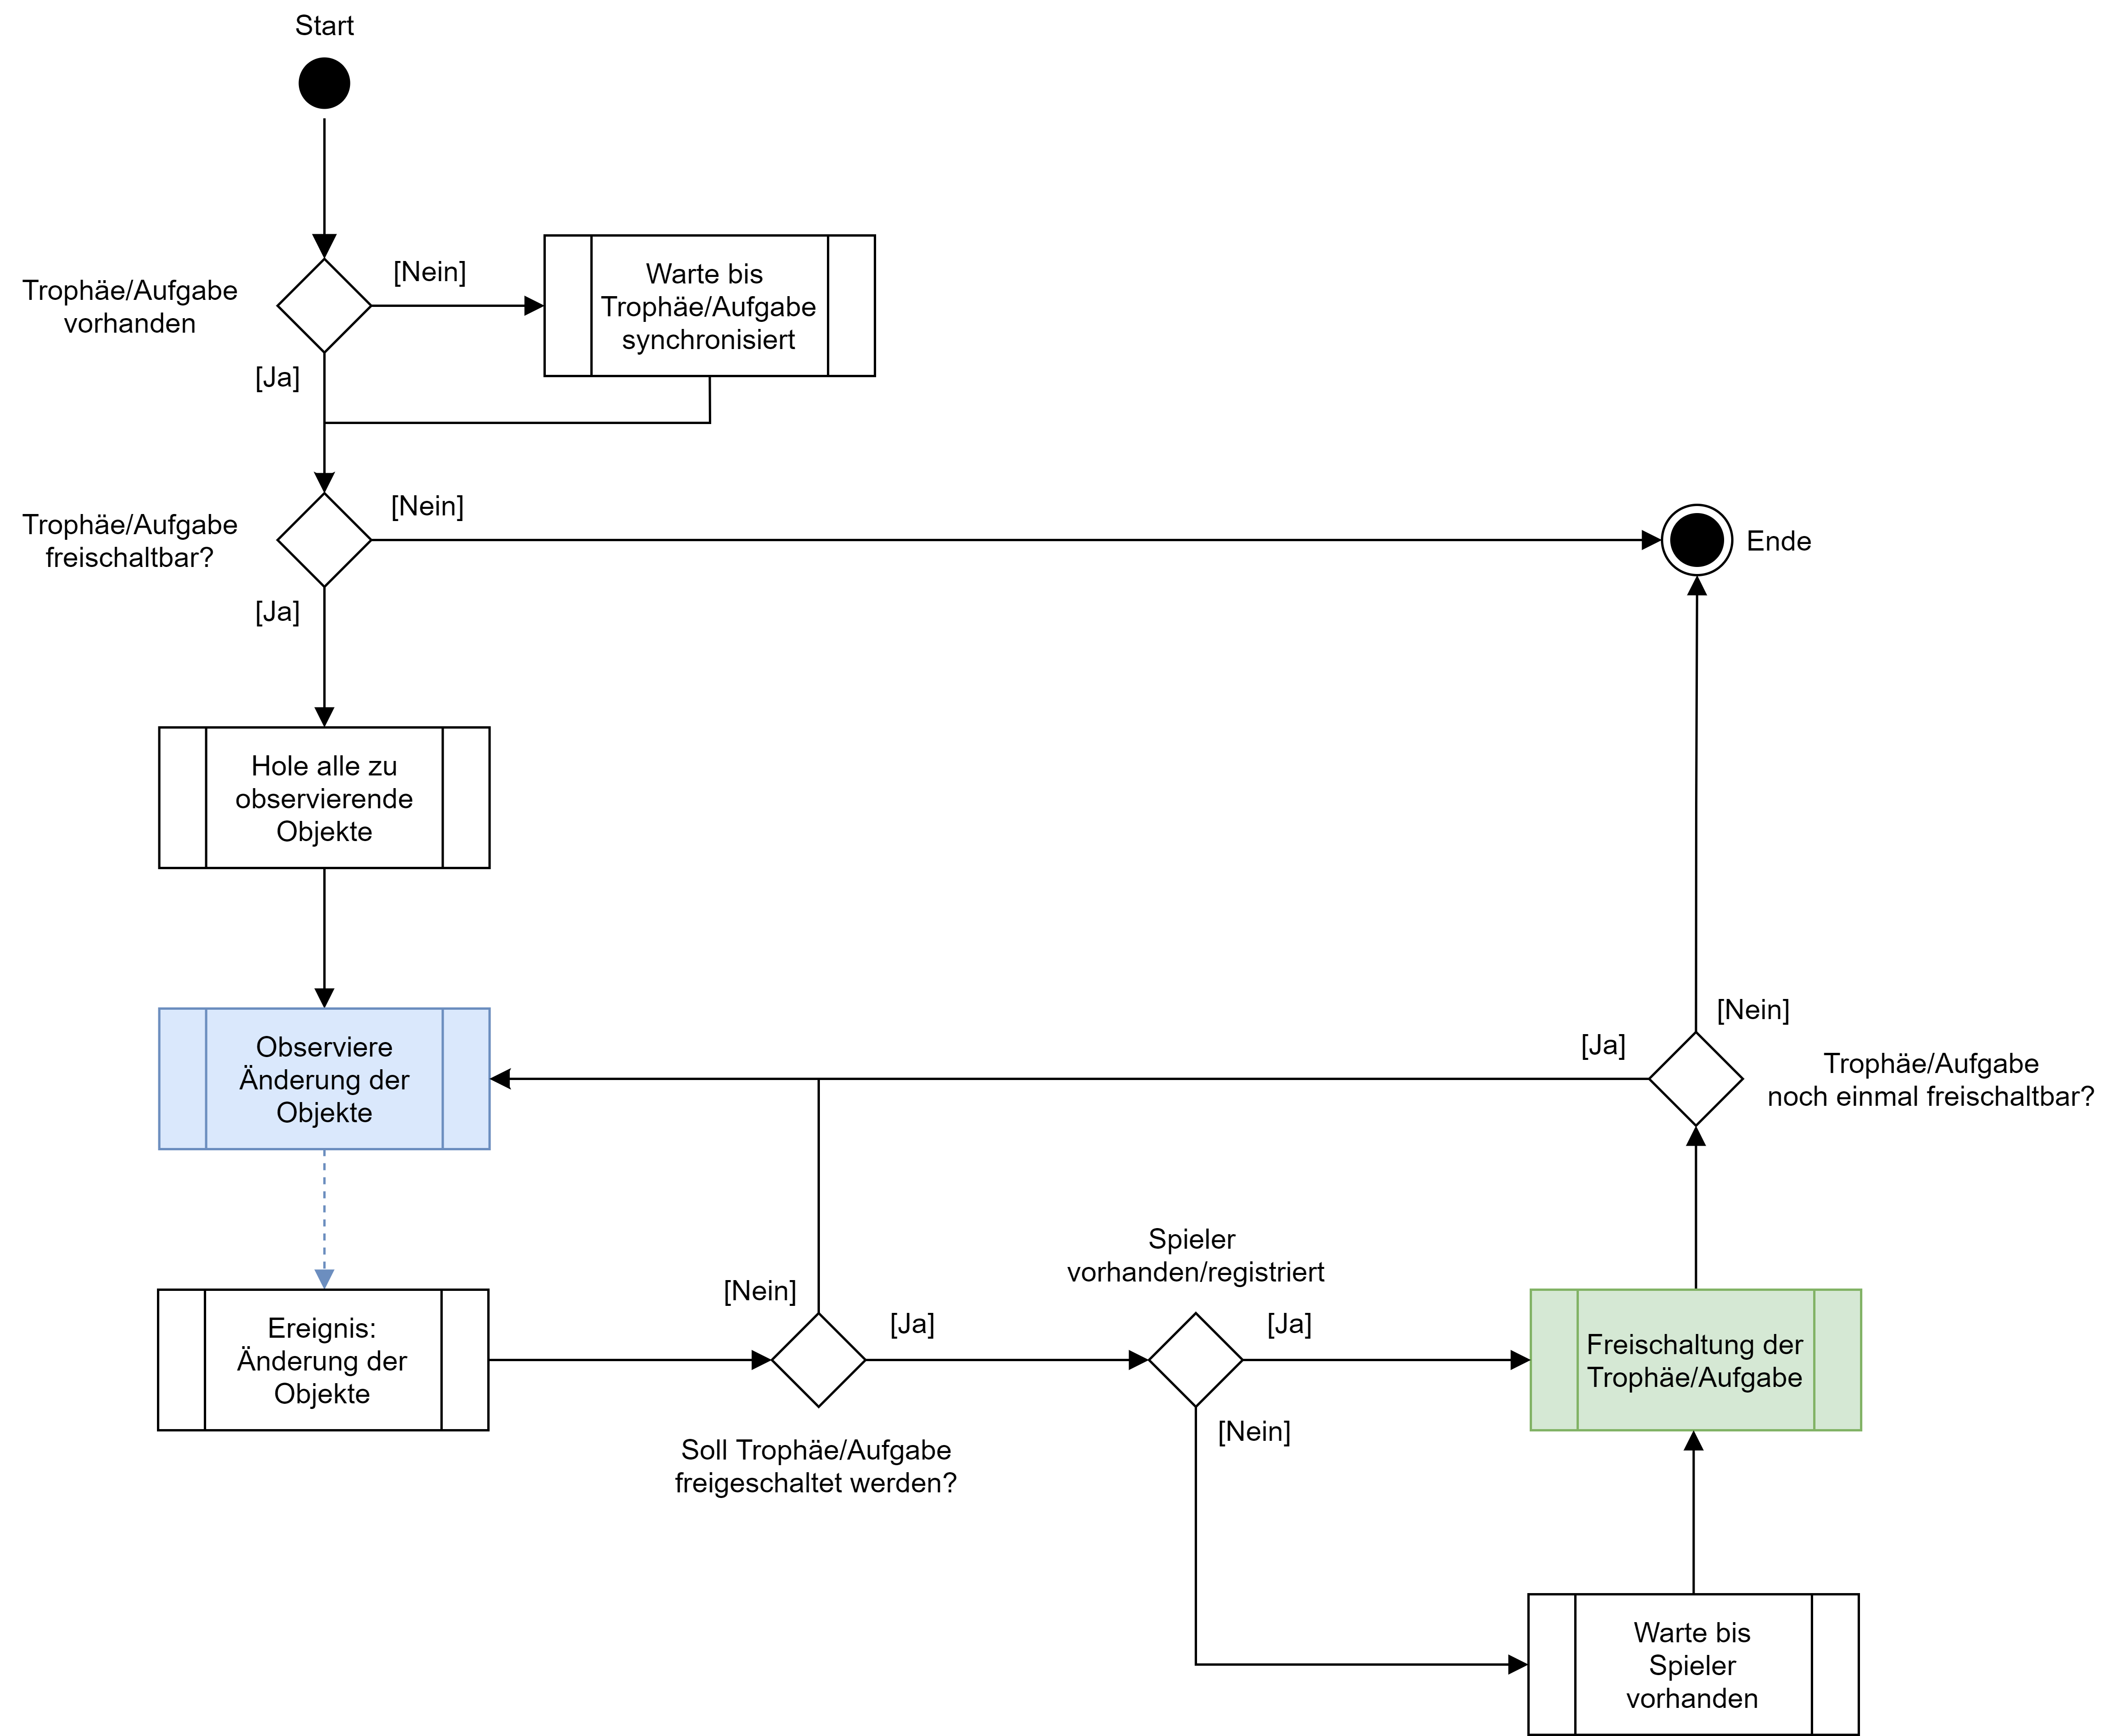
\includegraphics[width=1\linewidth]{46-repository-listener.png}
    \caption{Ein Algorithmus für die datenbasierte Freischaltung von Trophäen und Aufgaben.}\label{fig:repository-listener}
\end{figure}

Wie in \Cref{fig:repository-listener} gezeigt, werden beim Start der App die jeweiligen Observer initialisiert. Falls die referenzierten Trophäen oder Aufgaben zu diesem Zeitpunkt noch nicht synchronisiert wurden, wird die entsprechenden \texttt{Coroutine} pausiert, bis eine Synchronisation dieser Objekte erfolgt ist. Im Folgenden kann geprüft werde, ob die Trophäe oder Aufgabe bereits durch den Nutzer freigeschaltet wurde. Wurde eine Trophäe bereits erreicht, oder eine nicht wiederholbare Aufgabe abgeschlossen, so finalisiert der Algorithmus seine Ausführung. Kann die Errungenschaft stattdessen durch den Nutzer erreicht werden, so werden die dafür relevanten Objekte aus der Datenbank geholt, und ein entsprechender asynchroner \texttt{Flow} erstellt, welche alle Änderungen an diesen zu observierenden Objekten übermittelt. Im Falle einer Änderung kann nun geprüft werden, ob alle Kriterien für die Freischaltung erfüllt sind. Sind alle Kriterien erfüllt, so wird geprüft, ob ein Spieler bereits für das Spiel registriert ist, um die Freischaltung durchzuführen und die entsprechenden Boni zuzuweisen. Sollte ein Spieler zu diesem Zeitpunkt noch nicht registriert sein, so wird die Ausführung erneut pausiert, bis der Spieler eine Registrierung für das Spiel durchgeführt hat. Nach erfolgreicher Freischaltung der Errungenschaft endet die Ausführung, für den Fall das es sich um eine Trophäe oder einmalige Aufgabe handelt. Kann die Aufgabe erneut freigeschaltet werden, so führt der Algorithmus seine Observation der Änderung an den Datenbank-Objekten fort. \newpage Durch den beschriebenen Algorithmus konnten alle datenbasierten Errungenschaften implementiert werden. Beispielsweise wird bei der Trophäe \enquote{THE MAP IS HOT} bei jeder Änderung des Spielers geprüft, ob dieser bereits 90 Minuten am Crowd Monitoring teilgenommen hat. Gleichzeitig konnten die QR-Code-basierten Aufgaben umgesetzt werden, indem Änderungen an den \texttt{ScannedQRCode}-Objekten gegenüber den referenzierten Aufgaben abgeglichen werden.

\subsection{Implementation von interaktionsbasierten Errungenschaften}

Da bestimmte Errungenschaften nicht von direkten Änderungen von Datenmodellen aus der Datenbank abhängen, sondern durch Interaktionen des Nutzers innerhalb der App bestimmt sind, lässt sich der in \Cref{subsection:gamification-repository-listener} vorgestellte Algorithmus auf diese Art von Trophäen und Aufgaben nicht anwenden. Daher wurde zu diesem Zweck ein weiterer Algorithmus entwickelt, der allerdings wie im Folgenden vorgestellt auf die gleichen Prinzipien und Strukturen zurückgreift.

\begin{figure}[H]
    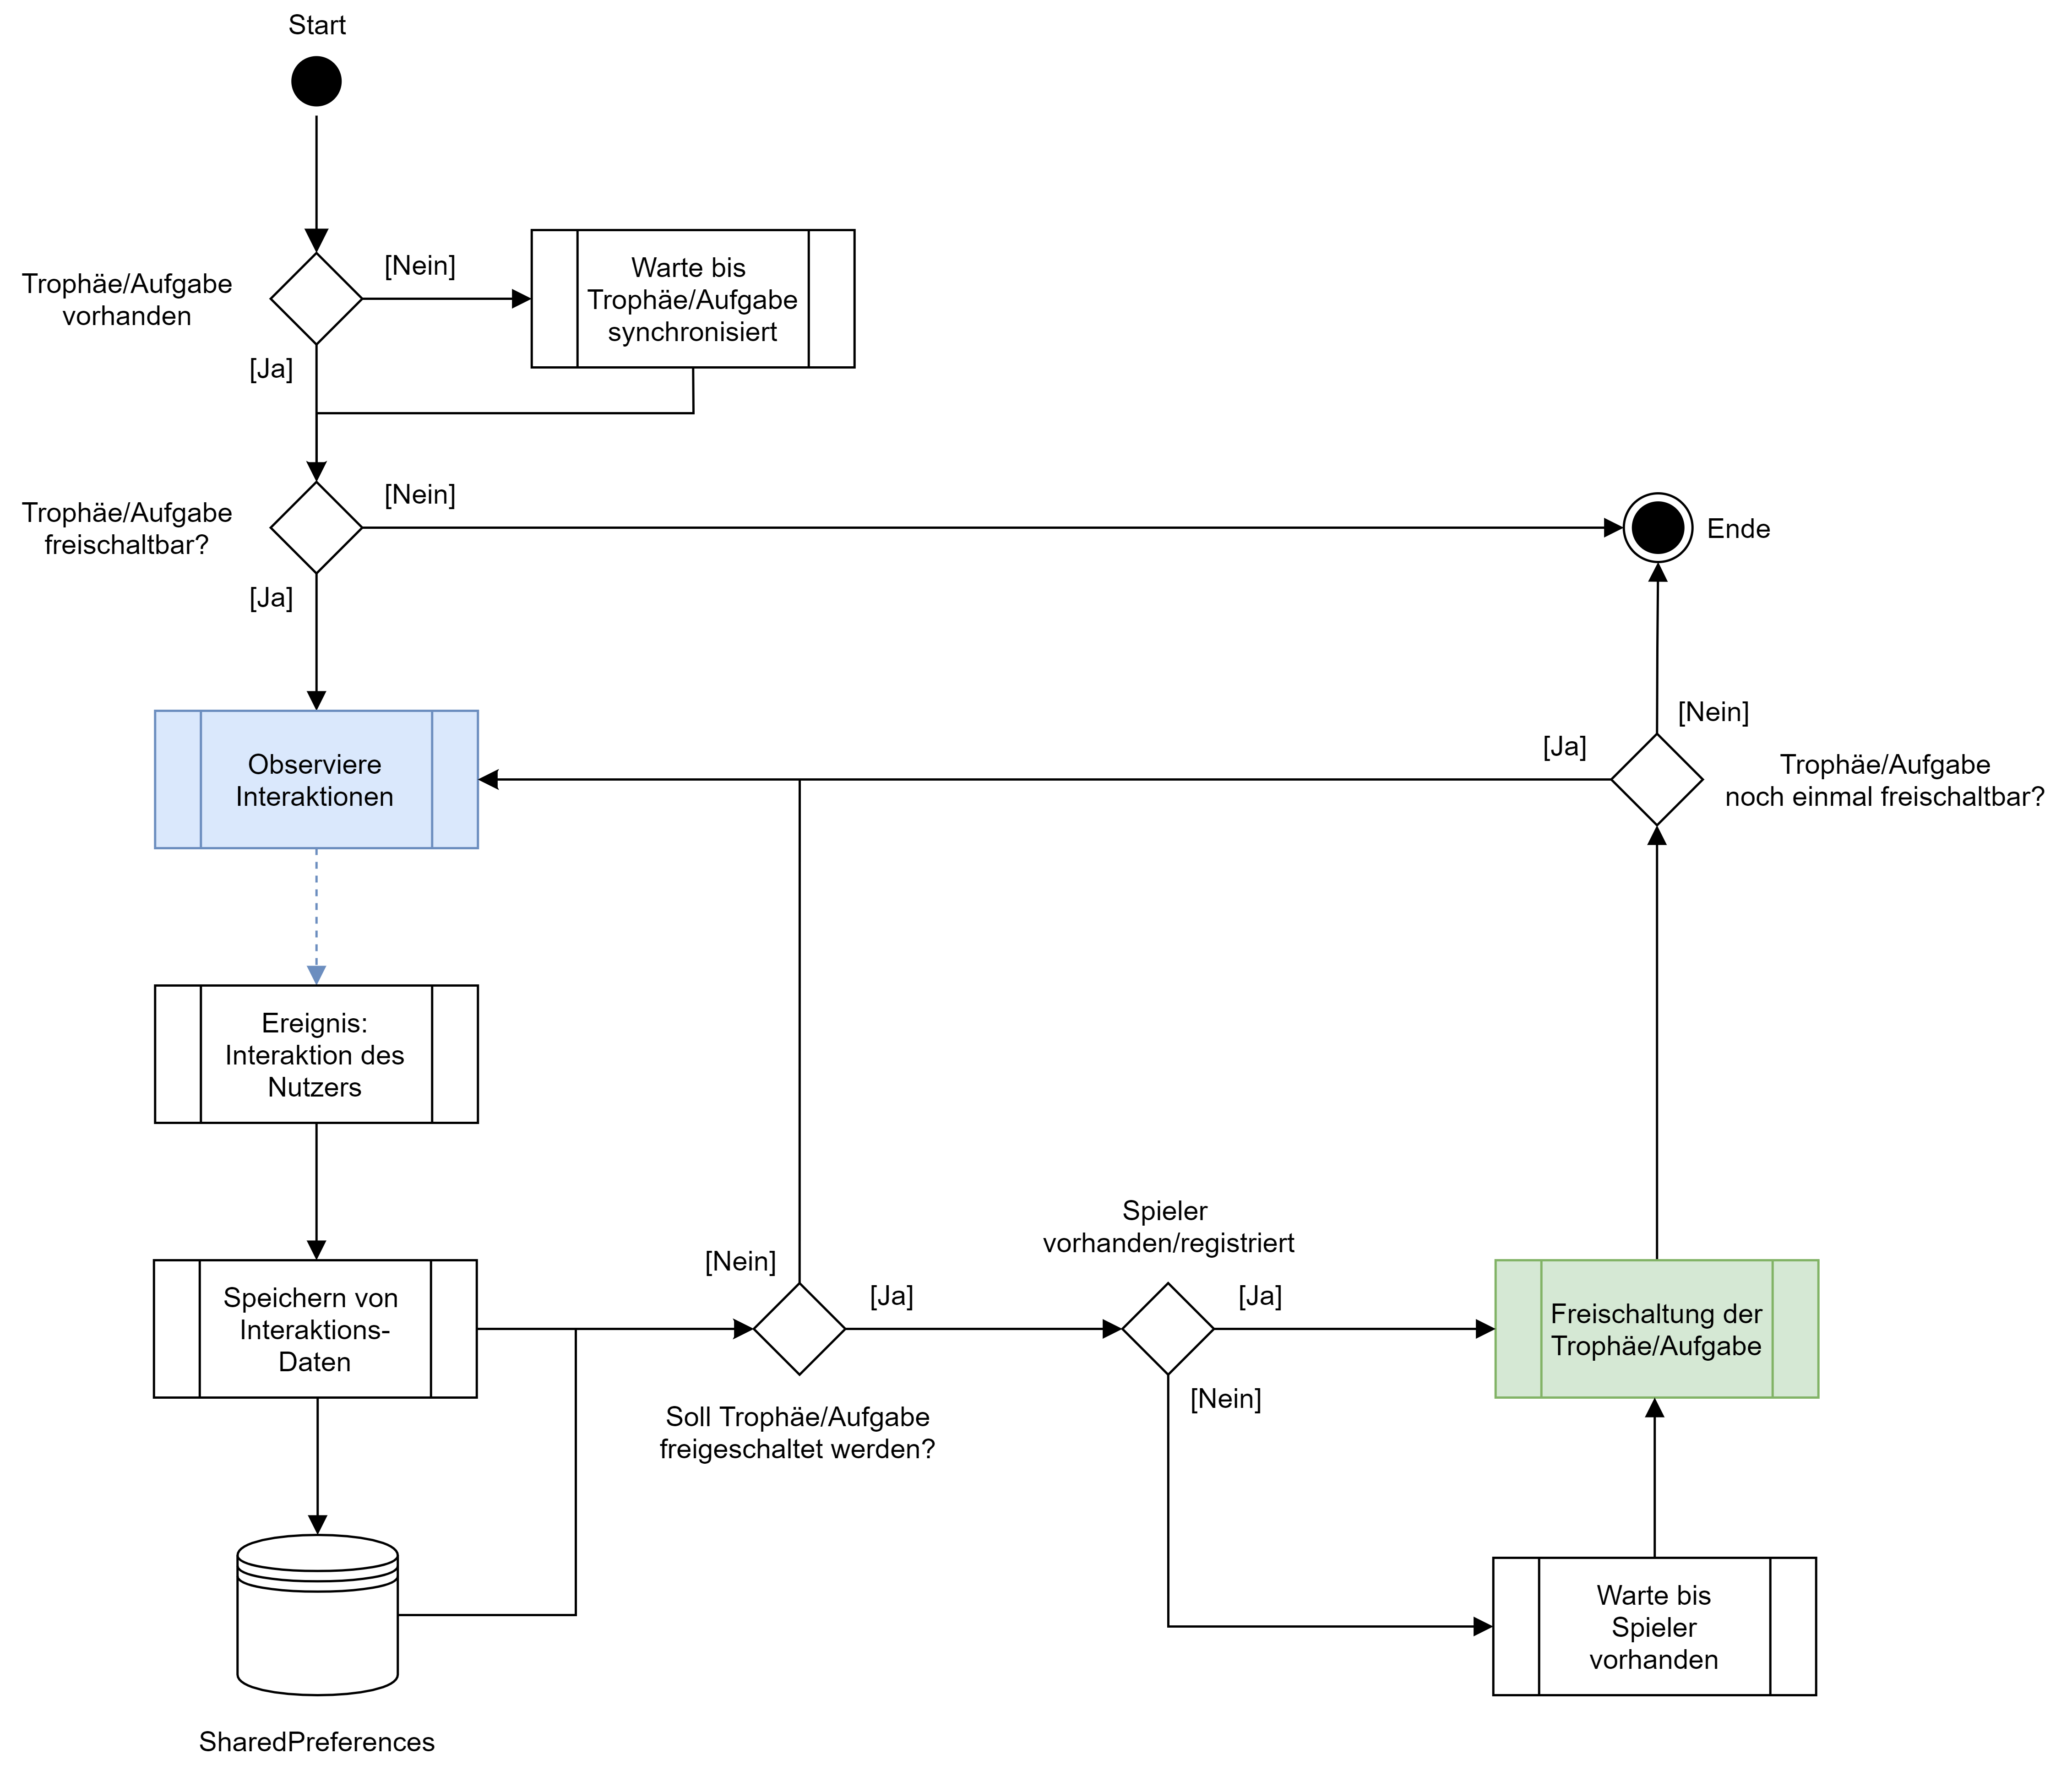
\includegraphics[width=1\linewidth]{47-interaction-listener.png}
    \caption{Ein Algorithmus für die interaktionsbasierte Freischaltung von Trophäen und
    Aufgaben.}\label{fig:interaction-listener}
\end{figure}

Der in \Cref{fig:interaction-listener} gezeigte Algorithmus ähnelt dem in \Cref{subsection:gamification-repository-listener} vorgestellten Algorithmus sehr stark, unterscheidet sich jedoch in wesentlichen Punkten. Anstelle von Änderungen an Datenmodellen bildet sich der asynchrone Datenstrom hierbei aus Interaktionen des Nutzers innerhalb der App. Diese Interaktionen werden durch eine Vererbung der abstrakten Klasse \texttt{GameInteractionEvent} abgebildet und beinhalten beispielsweise die Identifikation der vom Nutzer betrachteten Ansicht. Ähnlich wie auch bei den \hyperref[subsection:gamification-repository-listener]{datenbasierten Errungenschaften} werden die Änderungen als asynchroner Datenstrom mittels \texttt{Flow} realisiert. Bei jeder Interaktion werden die relevanten Informationen anschließend persistent in den \texttt{SharedPreferences} gespeichert. Beispielsweise wird für die Trophäe \enquote{APP EXPLORER} eine Historie an besuchten Ansichten gespeichert, um zu ermitteln, ob ein Nutzer die 5 Hauptansichten der App aus \Cref{subsection:views} sowie dem QR-Code Scanner genutzt hat. Die Verwertung der Ereignisse sowie der nachfolgende Ablauf findet äquivalent zum Fall von \hyperref[subsection:gamification-repository-listener]{datenbasierten Errungenschaften} statt. 


\section{Integration und Testen}

Um die bestehende App mit allen Funktionalität ausgiebig testen zu können wurde im Rahmen der Entwicklung eine Reihe von Komponenten entwickelt. Anhand dieser Komponenten konnte der Entwicklungsprozess unterstützt und die korrekte Implementierung validiert werden. Zugleich war es möglich die Nutzung der App zwischen den verschiedenen Betriebssystemen iOS und Android zu testen, um unter anderen die korrekte Serialisierung von Daten in einem einheitlichen Format sicherzustellen.

\paragraph{Testen der Datenbankfunktionalität} Für das Testen der Datenbankfunktionalität wurde der Datensatz der vorangegangenen Jahre aufbereite, und in ein Format gebracht, welches von der neuen Datenbankstruktur genutzt werden konnte. Zu diesem Zweck wurden sogenannte \enquote{Daten-Initialisierer} programmiert, welche die Daten aus \texttt{.json}-Dateien einlesen und beim erstmaligen Start der App in die lokale Datenbank importieren. Des Weiteren war es nötig, für einige Modelle neue Daten zu erstellen, da diese am Veranstaltungstag dynamisch erzeugt werden. Beispielsweise werden die Informationen der Beacons durch das Crowd-Monitoring-Framework ermittelt und anschließend in die Datenbank geschrieben, um darauf basierend eine Heatmap in der Kartenansicht zu erzeugen. Aus diesem Grund wurden Test-Skripte entwickelt, welche Bestandteil des iOS-Repository sind. Mit den vorliegenden Daten konnte die Nutzung der Datenbank getestet und die Einbindung von UI-Komponente validiert werden. 

\paragraph{Integration der Synchronisation} Zur persistenten Speicherung der App-Daten wird das Framework Couchbase verwendet. Daten werden in einzelnen Dokumenten gespeichert und könnten automatisiert zwischen den Geräten synchronisiert werden. Dafür ist es notwendig eine entsprechende Synchronisation zu konfigurieren. Um die Probleme des Datenschutzes von nutzerbezogenen Daten zu beheben, wurde im Rahmen der Entwicklung des Datenbank-Framework eine Unterteilung in öffentliche (\texttt{shared}) und persönliche (\texttt{personal}) Datenmodelle eingeführt. Während die öffentlichen Daten unveränderbar sind und für alle Nutzer zur Verfügung stehen, werden die persönlichen Daten nur von einem Nutzer geschrieben und können von anderen Nutzern nicht eingesehen werden. Zur Realisierung dieser Struktur war es notwendig die Synchronisation der Dokumente ebenfalls entsprechend der beiden Szenarien zu unterteilen. Die Durchführung der Synchronisation übernimmt dabei ein sogenannter Replikator, welcher die Konfiguration sowie den Endpunkt spezifiziert. Im Falle der öffentlichen Daten wird dabei für alle Nutzer eine einheitliche Konfiguration verwendet. Für die persönlichen Daten wird hingegen für jeden Nutzer bei der Spieler-Registrierung eine eigene Konfiguration aus Nutzername und Password erzeugt. Diese Anmeldeinformationen können im Folgenden genutzt werden, um sich beim Endpunkt zu authentifizieren. Die Synchronisation der Dokumente verläuft anschließend in einem separaten \enquote{Channel}, auf den nur der Nutzer Zugriff erhält. 

\newpage

\paragraph{Deployment der Anwendung} Zum Testen der Replikation wurde ein, aus der Entwicklung des Couchbase-Framework entstandenes, Container Deployment auf der Basis von \texttt{Docker}\footnote{Docker. \url{https://www.docker.com/}} verwendet. Dieses Setup entspricht ebenfalls dem finalen Deployment wie es bei der Veranstaltung genutzt werden wird. Dabei werden folgende Services genutzt: 

\begin{itemize}
    \item \textbf{Couchbase Server}, die zentrale Datenbank-Anwendung welche die gespeicherten Daten mittels des Couchbase-Framework verwaltet.
    \item \textbf{Couchbase Sync Gateway}, eine Schnittstelle für mobile Apps um die Synchronisation von Dokumenten durchzuführen. Dieser Service dient als Endpunkt für die iOS- und Android-Apps. Dabei werden Dokumente von der Sync Gateway an den Couchbase Server übermittelt. Die Sync Gateway dient somit als ein Proxy für den Couchbase Server.
    \item \textbf{Registration Service}, eine Server-Applikation, welche zur Registrierung eines neuen Spielers genutzt wird. Dabei wird für jeden Spieler ein entsprechender Nutzer in Sync Gateway erstellt, welcher im Folgenden genutzt wird um private Dokumente zu synchronisieren.
    \item \textbf{Sync Service}, welcher die Daten der OUTPUT.DD-Website mit dem Couchbase-Server synchronisiert und automatisierte Aufgaben wie die Erstellung einer Spielerliste übernimmt. Gleichzeitig stellt der Sync Service ein Web-Interface zur Verfügung, um ein Abbild der aktuellen Datenbank zu generieren oder eine PDF-Datei mit QR-Codes zu erstellen. 
    \item \textbf{Update Notifier}, ein Microservice, welcher den Sync Service von bestimmten Aktualisierungen in der Datenbank benachrichtigt.
\end{itemize}

Das Deployment kann durch die Verwendung von Docker Compose lokal auf dem Entwicklersystem oder auf einem beliebigen Server gestartet werden. Im Folgenden können die Endpunkte für die Replikation und die Registrierung referenziert und die Korrektheit der Replikator-Implementation zunächst lokal und im weiteren Verlauf auch anhand eines Remote-Servers geprüft werden. Eine Übersicht des Deployment ist in \Cref{fig:deployment} dargestellt.

\begin{figure}[H]
    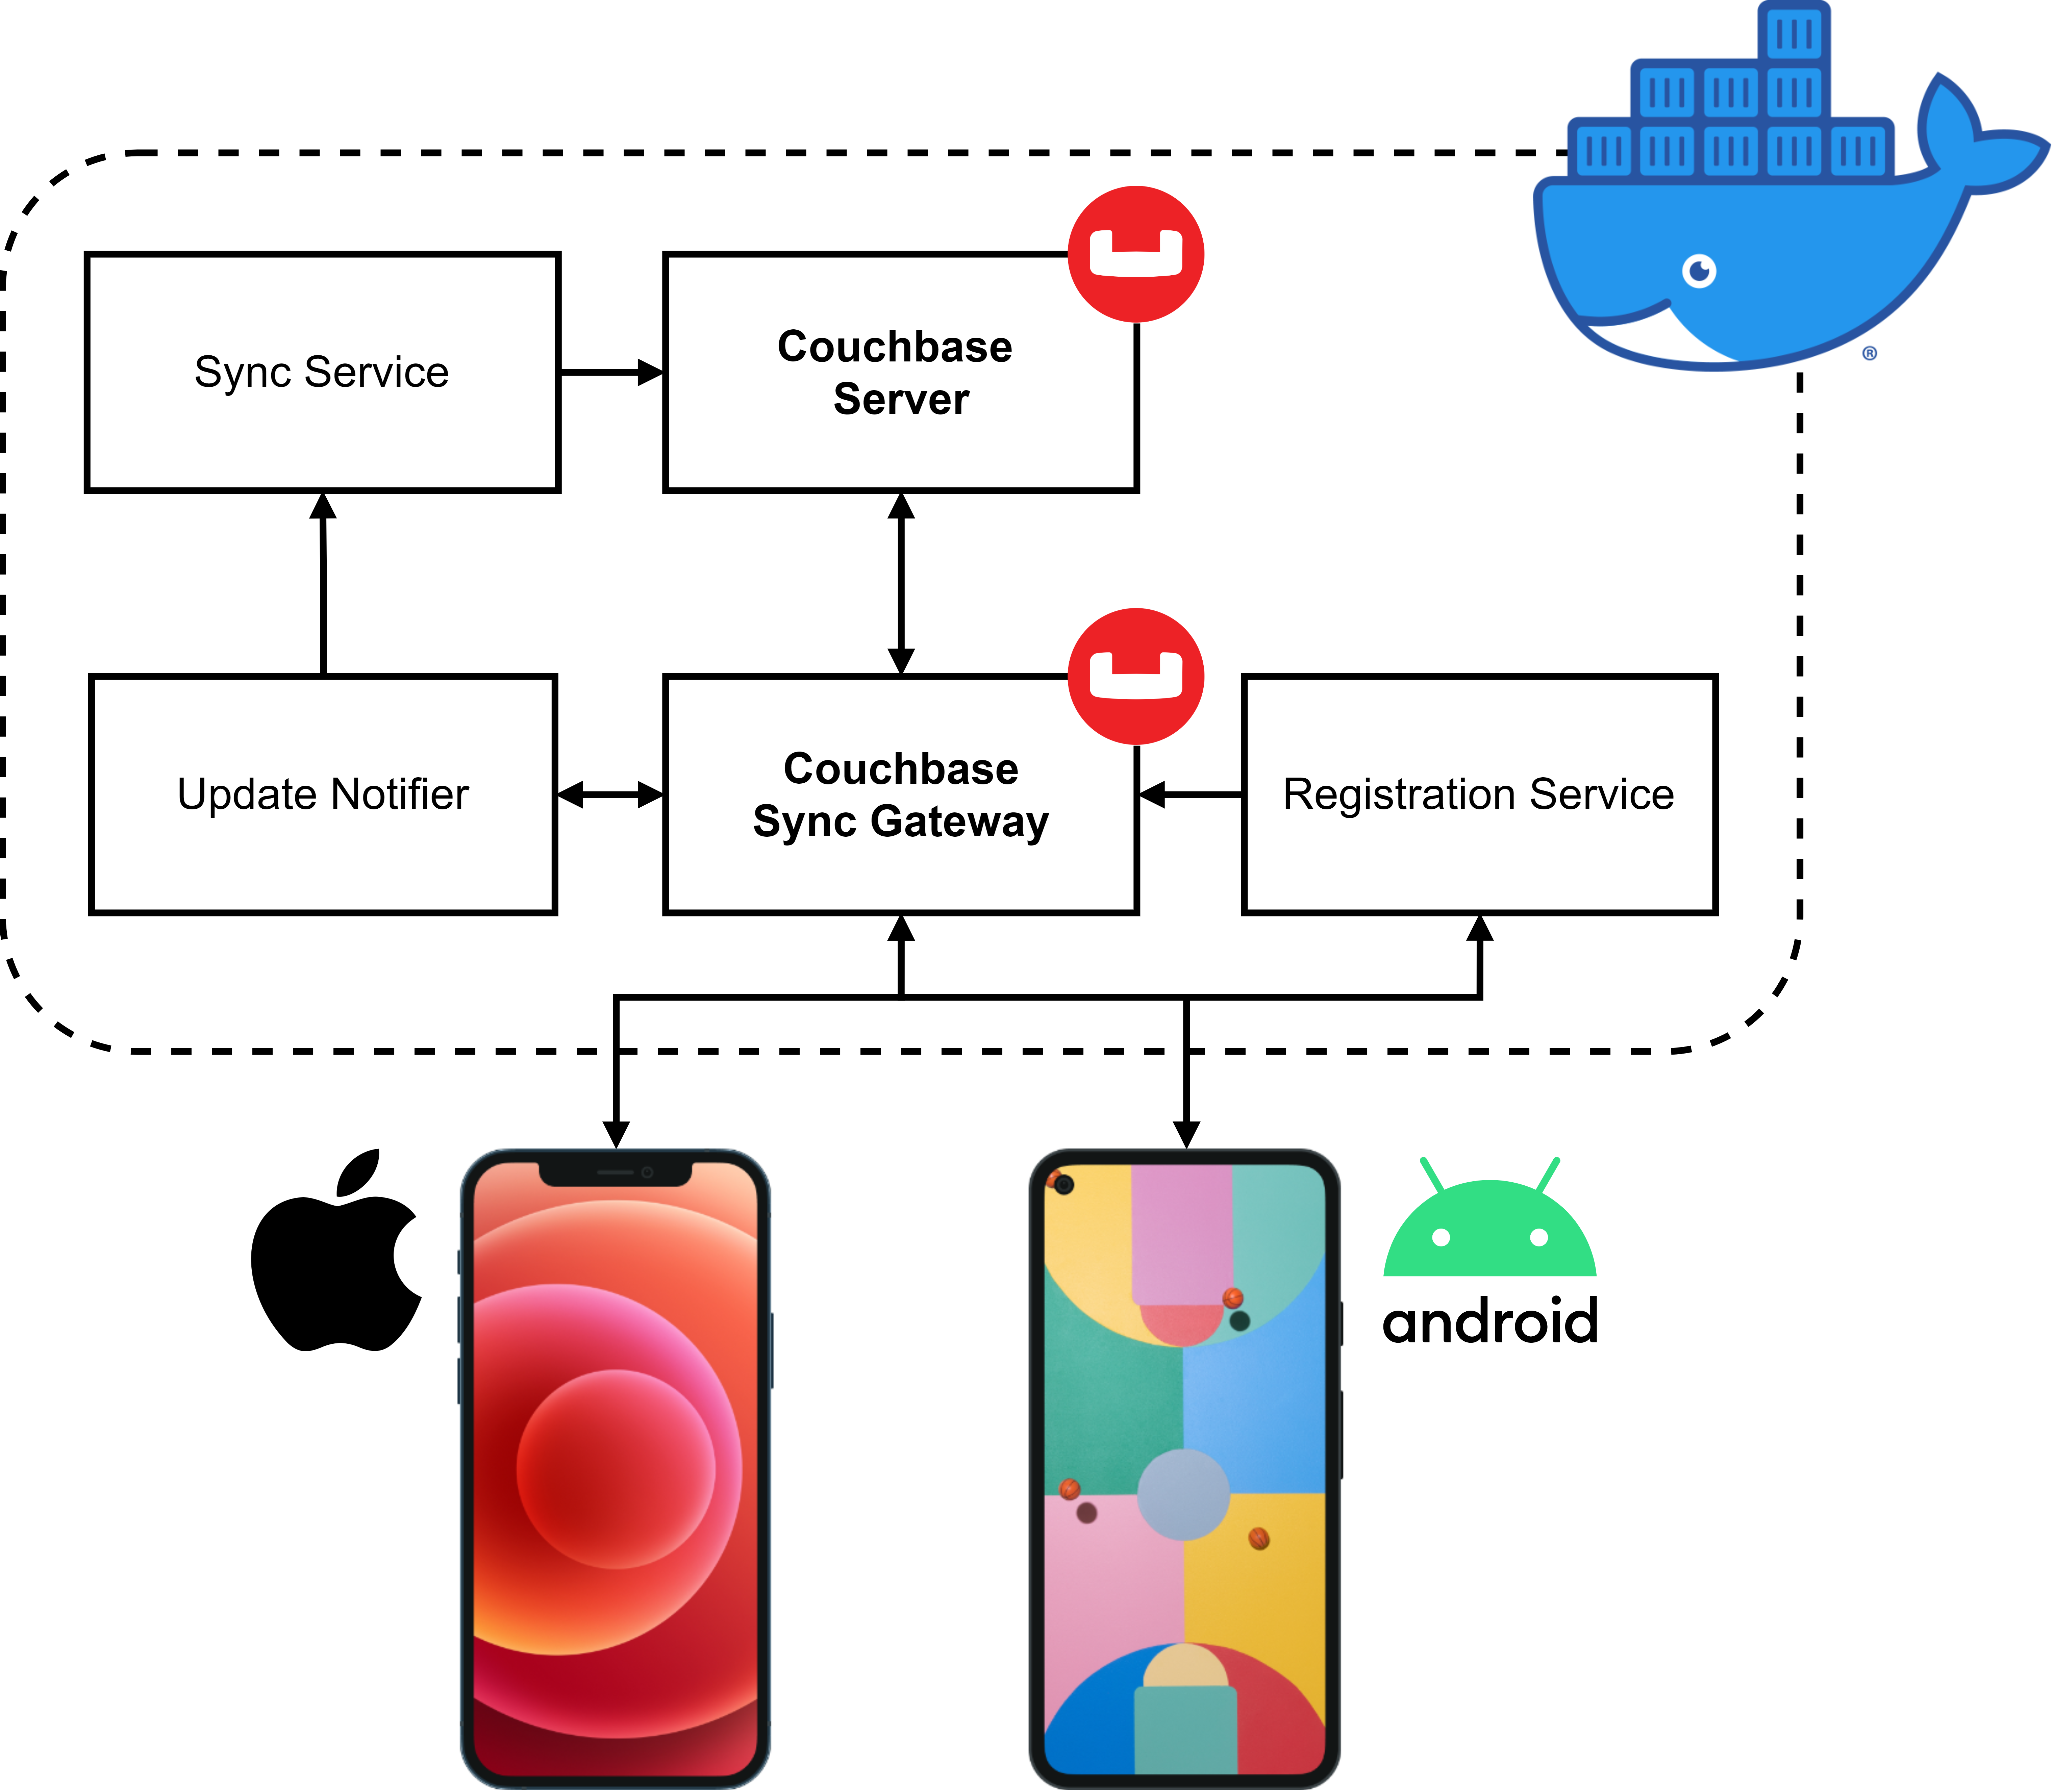
\includegraphics[width=0.75\linewidth]{48-deployment.png}
    \caption{Das Docker Deployment der App.}\label{fig:deployment}
\end{figure}